\documentclass[conference]{IEEEtran}
\IEEEoverridecommandlockouts
% The preceding line is only needed to identify funding in the first footnote. If that is unneeded, please comment it out.
\usepackage{cite}
\usepackage{amsmath,amssymb,amsfonts}
\usepackage{algorithmic}
\usepackage{graphicx}
\graphicspath{ {images/} }
\usepackage{textcomp}
\def\BibTeX{{\rm B\kern-.05em{\sc i\kern-.025em b}\kern-.08em
    T\kern-.1667em\lower.7ex\hbox{E}\kern-.125emX}}
\begin{document}

\title{Automatic Medical Coding for Neonatal Jaundice Using Ensemble Methods
}


\author{\IEEEauthorblockN{Scott Werwath}
\IEEEauthorblockA{
\textit{UC Berkeley}\\
sbw@berkeley.edu}
}

\maketitle

\begin{abstract}
This study explores the creation of a machine learning model to automatically identify whether a Neonatal Intensive Care Unit (NICU) patient was diagnosed with neonatal jaundice during a particular hospitalization based on their associated clinical notes. We develop a number of techniques for text preprocessing and feature selection and compare the effectiveness of different classification models. We show that using ensembled decision tree classification with AdaBoost outperforms support vector machines (SVM), the current state-of-the-art technique for neonatal jaundice coding.
\end{abstract}

\section{Introduction}
\subsection{Medical Coding}\label{AA}
In the course of normal clinical operations, healthcare providers are often required to \textit{code} patient records. The process of coding involves taking all data associated with a single patient case and abstracting out a set of standardized alphanumeric codes where each unique code is associated with a unique diagnosis or medical procedure. These codes are used for a variety of applications, including medical billing, as labels in statistical analysis of medical datasets, as features in clinical decision making, and as tags in information retrieval systems. 

While many coding schemes exists, the most widely used is the International Classification of Diseases, 9\textsuperscript{th} Revision (ICD-9) [SLEE]. Each ICD-9 codes consists of 3 to 5 alphanumeric characters which represents either a diagnosis or a procedure.

In actual clinical practice, coding is performed manually by professional medical coders. This process is both time-intensive and error-prone due to the fact that patient health records contain a large amount of data in free-text narrative format which is difficult to interpret quickly for both humans and computers [TANGE]. 

A system for automatic coding would have the potential to substantially decrease the number of man-hours required to process clinical cases, but building such a system requires the ability to extract important information from free-text reports. To this end, the application of natural language processing (NLP) and machine learning (ML) techniques to clinical texts show much promise [MEYSTRE].

\subsection{Neonatal Jaundice}\label{AA}
Neonatal jaundice, also called neonatal hyperbilirubinemia, is a yellow discoloration of the skin due to elevated bilirubin in a neonate's (infant's) blood. Transient neonatal jaundice is somewhat common in infants and usually carries little risk. However, untreated jaundice can put premature or otherwise ill infants at great risk of developing permanent neurological impairments [LANTZY]. Additionally, it has been shown that the diagnosis of neonatal jaundice is a risk factor for both mortality and rehospitalization [ESCOBAR]. 

Both the risk factors associated with and the relative prevalence of neonatal jaundice make it an excellent subject for study using machine learning techniques; the risk factors provide the motivation, while the prevalence provide a wealth of data to be analyzed.

\section{Related Work}
The past few years have seen a meteoric rise in the application of natural language processing (NLP) in the medical field [WOLNIEWICZ]. The cost of analyzing medical documents, both monetary and time, has motivated efforts to automate many manual tasks in the analysis and processing of medical texts.

Given both the importance and time-intensive nature of medical coding, many scientists have started developing techniques for automated coding. [MEYSTRE]. For most of these attempts, the task was domain-specific (i.e. attempting to predict a single ICD code or a small set of related codes) and utilized a relatively small dataset. 

At least one attempt has been made to use deep learning (namely character-level recurrent neural networks) to build more general coding models, but with limited success [SHI]. The main limitation with this method is that deep learning models require a large amount of data to train [CHEN], but even a large clinical dataset may only contain a few examples of case files with any given ICD code. Additionally, since the ICD-9 standard contains over 14,000 different codes. Treating coding as a simple multi-class classification problem with 14,000 different classes is infeasible.

More successful automated coding models have utilized non-deep machine learning techniques such as support vector machines (SVMs) [VAPNIK] and focus on training a model to detect the presence of a single ICD code or class of related codes. Some of these methods also leverage structured data stored in health records in addition to free-text narratives [FERRAO].

At least one previous attempt has been made to build an automatic coding model for neonatal jaundice using an SVM on the text of clinical notes [MARAFINO]. Our research improves on this model by introducing a number of preprocessing stages. We also explore and compare alternative classification techniques and analyze their efficacy.

No matter the exact method for extracting medical codes from free-text, two common NLP challenges must be solved. First, one must represent free-text in an appropriate feature space (usually as a vector). Second, one must train a model to accurately classify patient records based on the selected features. 

\section{Methodology}
\subsection{Dataset and Data Extraction}\label{AA}
The Medical Information Mart for Intensive Care III (MIMIC-III) dataset contains complete anonymized records from over 53,000 ICU stays [JOHNSON]. These records were gathered from hospital records from the Beth Israel Deaconess Medical Center in Boston, Massachusetts between 2001 and 2012. Of these records, 7870 correspond to neonates admitted between 2001 and 2008. 

Each hospital stay in the MIMIC-III dataset is assigned a unique HADM\_ID identifier which can be used to cross-reference associated data back their associated hospitalization.

In order to find all patients who were diagnosed with neonatal jaundice, we found all HADM\_IDs that were labeled with an ICD-9 code associated with neonatal jaundice. A list of such codes are shown in Table~\ref{tab1}. 
\begin{table}[htbp]
\caption{ICD-9 Codes for Neonatal Jaundice}
\begin{center}
\begin{tabular}{cc}
\textbf{ICD-9 Code}&\textbf{Description} \\
\hline
\textbf{773.0} & Hemolytic disease, RH isoimmunization \\
\textbf{773.1} & Hemolytic disease, ABO isoimmunization \\
\textbf{773.0} & Hemolytic disease, unknown \\
\textbf{774.1} & Perinatal jaundice, excessive hemolysis \\
\textbf{774.2} & Neonatal jaundice, preterm delivery \\
\textbf{774.30} & Neonatal jaundice, delayed conjugation \\
\textbf{774.31} &  Neonatal jaundice, delayed conjugation, other \\
\textbf{774.39} & Other jaundice \\
\textbf{774.6} & Unspecified fetal and neonatal jaundice \\
\end{tabular}
\label{tab1}
\end{center}
\end{table}
In total, 7092 hospitalizations were of neonates. Of these, 2868 stays were associated with a neonatal jaundice diagnosis and served as positive examples. We also selected the remaining 4224 non-jaundice NICU stays as negative examples.

For each relevant hospitalization, we concatenated all ICU notes, including nursing notes, radiology reports, physician progress notes, and discharge summaries into a single string of text called a \textit{noteset}. This string served as the raw data to be preprocessed and then classified. 
\subsection{Data Preprocessing}\label{AA}
Preprocessing of raw text is an extremely important element of any NLP model, especially in the task of classification [HADDI]. In fact, the preprocessing of raw text is a form of manual feature selection, in which we are able to choose what parts of the document are to be given to the classifier [FATIH].

The first stage of our preprocessing algorithm is \textit{cleaning}, in which punctuation and other extraneous characters are stripped from the raw text. In addition to punctuation, numbers are also removed from the noteset. While numbers are often left in classifiers for medical texts, later cross-validation indicated that they were low-information for this particular task. Finally, we also remove anonymization indicators from the text of the doument. The indicators are special flags left to indicate that confidential patient data had been redacted from the noteset at that point in the text, and generally contained information that was irrelevant for classification such as dates, names, and phone numbers.

After the noteset is cleaned, it is \textit{tokenized}, or split into a stream of individual words. The next series of preprocessing steps act on individual words or multiword phrases, and they work to reduce the \textit{vocabulary}, or number of unique words, of our dataset. Vocabulary reduction often results in improved classification performance [MADSEN] because the model does not have to learn to classify low-information words or learn that synonymous words or phrases should be classified similarly. Depending on your representation of documents as vectors (e.g. one-hot encodings), vocabulary reduction corresponds directly to a dimensionality reduction of samples.

The first stage of vocabulary reduction is \textit{semantic mapping}, i.e. the replacement of synonymous words or phrases with a standard token [BANERJEE]. This allows the model to learn only one representation of the underlying concept rather than having to learn many. For this, we use a list of 727 common medical words and phrases [TAMANG] and use regular expressions to find and replace each of them in the notesets. Examples of such replacements can be found in Table~\ref{reptab}.
\begin{table}[htbp]
\caption{Example Replacements During Preprocessing}
\begin{center}
\begin{tabular}{ccc}
\textbf{Rule}&\textbf{Raw Text}&\textbf{Processed Text} \\
\hline
\textbf{Semantic Map} & "raises concern" & "RISK" \\
\textbf{Semantic Map} & "cannot rule out" & "RISK" \\
\textbf{Semantic Map} & "no evidence of" & "NEGEX" \\
\textbf{Semantic Map} & "rule out" & "NEGEX" \\
\textbf{Stemming} & "neonatal" & "neonat" \\
\textbf{Stemming} & "neonate" & "neonat" \\
\textbf{Stop Word Removal} & "the patient is" & "patient" \\
\textbf{Phrase Detection} & "heart attack" & "heart\_attack" \\
\end{tabular}
\label{reptab}
\end{center}
\end{table}

After semantic mapping, we apply \textit{stemming}, which is the process of reducing words to their root morpheme (see Table~\ref{reptab}). For this task, we use the Snowball stemming algorithm [PORTER]. Since different morphological variations of the same word (e.g. "neonatal" and "neonate") likely have similar meanings, stemming allows the model to learn  a single classification for all morphological forms for a word.

Next, \textit{stop words} were removed from the notesets. Stop words are common words such as "the" and "it" which convey no real semantic information. The removal of stop words from raw text has been shown to improve the performance of classification models due to their being low-information and useless for most classification tasks [SILVA]. 

Finally, collocations, or common multiword phrases, are detected and replaced with a single token. In order to automatically detect collocations in our corpus, we calculate the \textit{normalized pointwise mutual information} (NPMI) of every pair of words in the corpus [BOUMA]. The NPMI is given by \eqref{pmi}, where $x$ and $y$ are indicators for a two given words appearing in text, $p(x,y)$ is the probability of the two words appearing next to each other, and all probabilities are measured empirically from our corpus.
\begin{equation}
i_n(x,y) = \frac{-1}{\ln p(x,y)}\ln \frac{p(x,y)}{p(x)p(y)}\label{pmi}
\end{equation}
Intuitively, NMPI measures how much the the co-occurance of two words $x$ and $y$ differs from what we would expect if their occurrences were independent of each other. For word pairs in our corpus with high NMPI, we normalized co-occurances in raw text into a single token (see Table~\ref{reptab}).
\subsection{Document Representation}\label{AA}
In order to classify notesets, we have to represent them as vectors. While deeper methods (e.g. convolutional neural networks) are able to take word order into account, we choose to use a \textit{bag-of-words} (BoW) model in which we ignore the actual ordering of words in a document and instead simply count the number of occurrences of each unique word in the document. This has the benefit of greatly simplifying our document representation, but it throws away potentially valuable information contained in word ordering (e.g. "negative for cancer, positive for flu" and "positive for cancer, negative for flu" will have the same BoW representation). Despite this disadvantage, however, BoW representations work very well in practice for many applications.

A naive approach to BoW representation is a \textit{count vector}. In a count vector, each unique word is represented by a $V$-dimensional one hot encoding vector, where $V$ is the size of the vocabulary. A document is then represented by the sum (or sometimes average) of the one hot encoding of all the words in the document. The result is that, at each index in a document vector, the entry at index $i$ is the number of times the $i$\textsuperscript{th} word in the vocabulary occurs in the document.

A commonly used technique to improve upon the count vector representation to weight each entry by the term's \textit{inverse document frequency} (IDF), given in \eqref{idf}. $N$ is the total number of documents in the corpus, and the denominator represents the number of documents in the corpus where the word $t$ appears.
\begin{equation}
idf(t) = \log \frac{N}{|\{d \in D : t \in d\} |}\label{idf}
\end{equation}
The IDF measures the rarity of a word in a given corpus. From an information theoretic perspective, words with high IDF (i.e. rarer words) provide more information, so we want to give them more weight in our decision making process.

When we weight each count vector entry by its word's IDF and normalize appropriately, we get that each entry $t$ in the vector representation for document $d$ is given by \eqref{tfidf}.
\begin{equation}
tfidf(t, d) = \frac{|t' \in d : t' = t|}{|d|} idf(t)\label{tfidf}
\end{equation}
This value is called the \textit{term frequency-inverse document frequency} (TF-IDF), and a vector of these values is called a TF-IDF vector.

\subsection{Baseline SVM Models}\label{AA}
Reference [MARAFINO] demonstrates the use of a support vector machine (SVM) to perform automatic coding for neonatal jaundice. This study used a grid search to determine that a linear kernel with penalty hyperparameter of $C = 100$. This model was reimplemented, and our own grid search over relevant hyperparmeters with 10-fold cross-validation found those same settings to be optimal. This SVM model was used as a baseline to compare with the performance of new ensemble learning methods. 
\subsection{Ensemble Methods}\label{AA}
\textit{Ensemble learning} refers to the practice of training and using multiple machine learning models and combining their outputs into a final output via a "voting" system. Ensemble methods often provide better results than using a single model because they can reduce variance. When a set of models are trained with random samples of a dataset or on a random subset of features, we are essentially sampling from the space of possible classifiers. By taking many samples and averaging their results, we reduce our reliance on the particularities of any one classifier and therefore reduce variance [DIETTERICH].

We used the sklearn package [PEDREGOSA] to implement two ensembled classifiers: AdaBoost with decision trees [ZHU] and bagged decision trees [BREIMAN]. 

AdaBoost 
\subsection{Evaluation}\label{AA}

\section{Results}
The performance of the baseline classifier from [MARAFINO], our implementation of SVM, and the two ensembled classifiers are summarized in Table~\ref{restab}
\begin{table}[htbp]
\caption{Performance of Various Classifiers}
\begin{center}
\begin{tabular}{ccccc}
\textbf{Classifier}&\textbf{Accuracy}&\textbf{Precision}&\textbf{Recall}&\textbf{F\textsubscript{1} Score} \\
\hline
\textbf{SVM (Marafino et al.)} & 0.898 & 0.908 & 0.853 & 0.884 \\
\textbf{SVM (reimplemented)} & 0.857 & 0.872 & 0.888 & 0.880 \\
\textbf{AdaBoost Trees} & \textbf{0.907} & \textbf{0.923} & 0.846 & 0.883 \\
\textbf{Bagged Trees} & 0.902 & 0.897 & \textbf{0.941} & \textbf{0.919} \\

\end{tabular}
\label{restab}
\end{center}
\end{table}
\section{Discussion}
\section{Conclusion}

\subsection{Figures and Tables}
\paragraph{Positioning Figures and Tables} Place figures and tables at the top and 
bottom of columns. Avoid placing them in the middle of columns. Large 
figures and tables may span across both columns. Figure captions should be 
below the figures; table heads should appear above the tables. Insert 
figures and tables after they are cited in the text. Use the abbreviation 
``Fig.~\ref{fig}'', even at the beginning of a sentence.

\begin{table}[htbp]
\caption{Table Type Styles}
\begin{center}
\begin{tabular}{|c|c|c|c|}
\hline
\textbf{Table}&\multicolumn{3}{|c|}{\textbf{Table Column Head}} \\
\cline{2-4} 
\textbf{Head} & \textbf{\textit{Table column subhead}}& \textbf{\textit{Subhead}}& \textbf{\textit{Subhead}} \\
\hline
copy& More table copy$^{\mathrm{a}}$& &  \\
\hline
\multicolumn{4}{l}{$^{\mathrm{a}}$Sample of a Table footnote.}
\end{tabular}
\label{tab2}
\end{center}
\end{table}

\begin{figure}[htbp]
\centerline{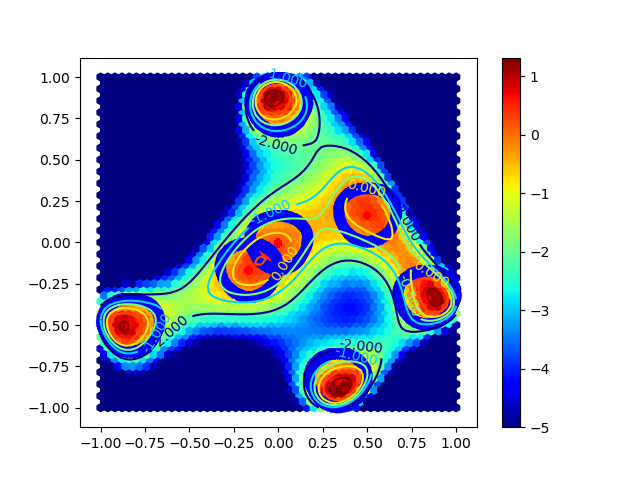
\includegraphics[scale=0.5]{fig1}}
\caption{Example of a figure caption.}
\label{fig}
\end{figure}

Figure Labels: Use 8 point Times New Roman for Figure labels. Use words 
rather than symbols or abbreviations when writing Figure axis labels to 
avoid confusing the reader. As an example, write the quantity 
``Magnetization'', or ``Magnetization, M'', not just ``M''. If including 
units in the label, present them within parentheses. Do not label axes only 
with units. In the example, write ``Magnetization (A/m)'' or ``Magnetization 
\{A[m(1)]\}'', not just ``A/m''. Do not label axes with a ratio of 
quantities and units. For example, write ``Temperature (K)'', not 
``Temperature/K''.

\section*{References}

Please number citations consecutively within brackets \cite{b1}. The 
sentence punctuation follows the bracket \cite{b2}. Refer simply to the reference 
number, as in \cite{b3}---do not use ``Ref. \cite{b3}'' or ``reference \cite{b3}'' except at 
the beginning of a sentence: ``Reference \cite{b3} was the first $\ldots$''

Number footnotes separately in superscripts. Place the actual footnote at 
the bottom of the column in which it was cited. Do not put footnotes in the 
abstract or reference list. Use letters for table footnotes.

Unless there are six authors or more give all authors' names; do not use 
``et al.''. Papers that have not been published, even if they have been 
submitted for publication, should be cited as ``unpublished'' \cite{b4}. Papers 
that have been accepted for publication should be cited as ``in press'' \cite{b5}. 
Capitalize only the first word in a paper title, except for proper nouns and 
element symbols.

For papers published in translation journals, please give the English 
citation first, followed by the original foreign-language citation \cite{b6}.

\begin{thebibliography}{00}
\bibitem{b1} G. Eason, B. Noble, and I. N. Sneddon, ``On certain integrals of Lipschitz-Hankel type involving products of Bessel functions,'' Phil. Trans. Roy. Soc. London, vol. A247, pp. 529--551, April 1955.
\bibitem{b2} J. Clerk Maxwell, A Treatise on Electricity and Magnetism, 3rd ed., vol. 2. Oxford: Clarendon, 1892, pp.68--73.
\bibitem{b3} I. S. Jacobs and C. P. Bean, ``Fine particles, thin films and exchange anisotropy,'' in Magnetism, vol. III, G. T. Rado and H. Suhl, Eds. New York: Academic, 1963, pp. 271--350.
\bibitem{b4} K. Elissa, ``Title of paper if known,'' unpublished.
\bibitem{b5} R. Nicole, ``Title of paper with only first word capitalized,'' J. Name Stand. Abbrev., in press.
\bibitem{b6} Y. Yorozu, M. Hirano, K. Oka, and Y. Tagawa, ``Electron spectroscopy studies on magneto-optical media and plastic substrate interface,'' IEEE Transl. J. Magn. Japan, vol. 2, pp. 740--741, August 1987 [Digests 9th Annual Conf. Magnetics Japan, p. 301, 1982].
\bibitem{b7} R. Wolniewicz (2015). "Computer-assisted coding and natural language processing."
\end{thebibliography}

\end{document}
